\section{方法细节}

\subsection{整体框架}

Vision-Zero 的整体流程如 Figure~\ref{fig:visionzero-figure3} 所示，可以分为三个部分：

\begin{itemize}
    \item Strategic Game Environment：把 VLM 放入多角色游戏，要求不同角色根据自己的视觉输入和历史线索采取策略性行动。
    \item Label-free and Domain-agnostic Data Input：每局游戏只需要图像输入，不需要人工 QA。普通玩家看到原图，卧底看到空白图像或与原图存在差异的图像。
    \item Iterative Self-Play Optimization：线索阶段用自博弈奖励训练，决策阶段用可验证投票奖励训练，并根据阶段饱和状态动态切换。
\end{itemize}

\begin{figure}[H]
    \centering
    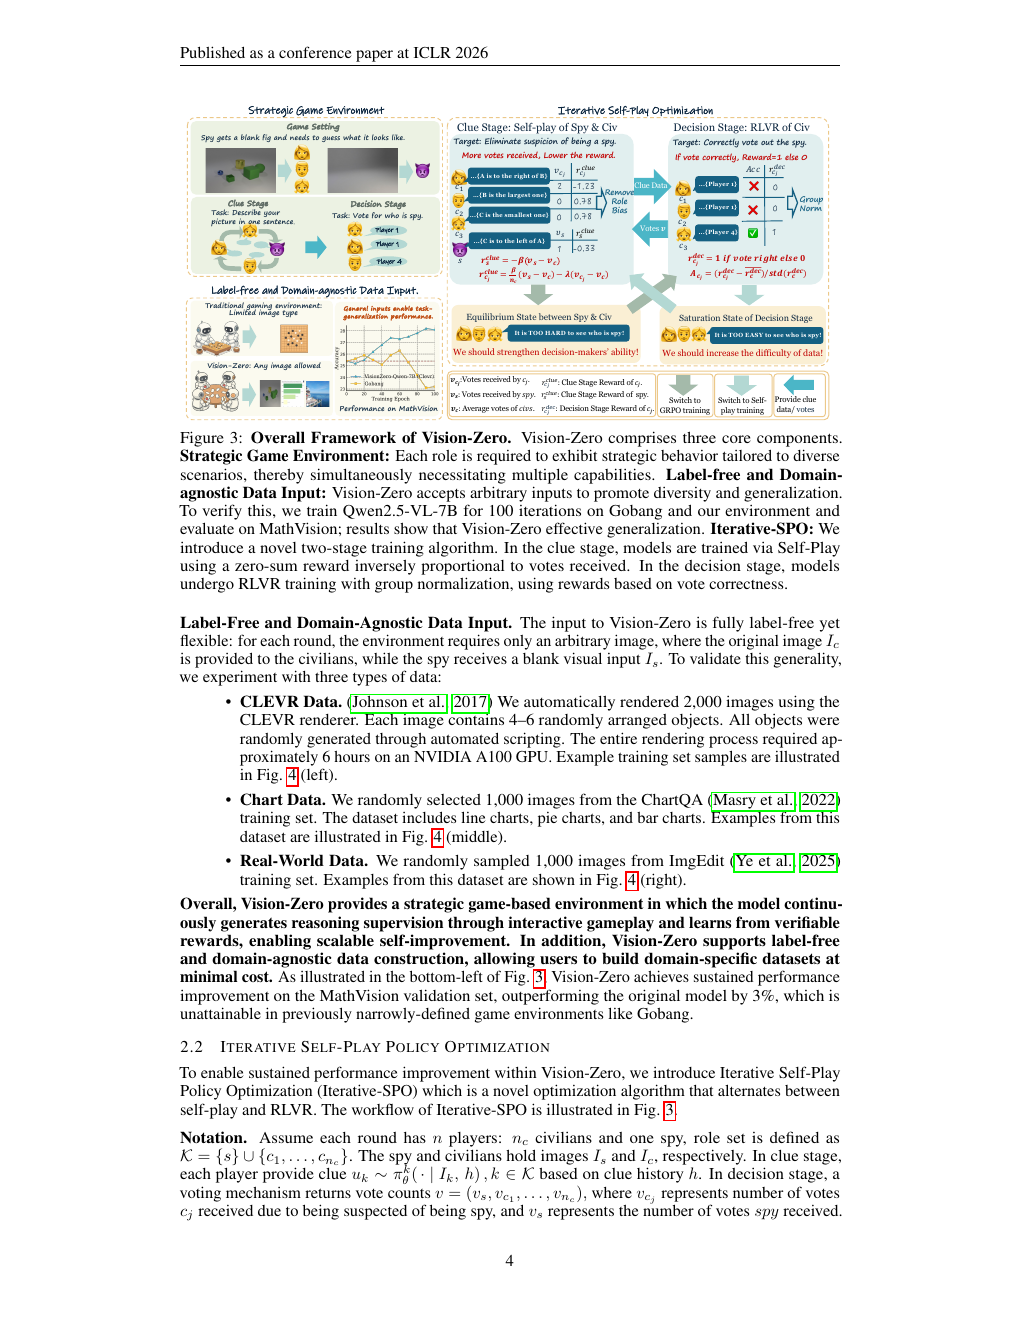
\includegraphics[width=0.95\textwidth]{figures/figure3_page.png}
    \caption{Vision-Zero 的游戏环境、无标签数据输入和 Iterative-SPO 训练流程。}
    \label{fig:visionzero-figure3}
\end{figure}

游戏本身包含两个阶段。第一是 clue stage：所有玩家知道自己的角色，然后观察图像并给出一句线索。普通玩家要给出真实、清晰、但不完全泄露图像内容的描述；卧底没有正常图像，因此必须根据前面玩家的线索推断图像内容，并给出看似合理的伪装线索。第二是 decision stage：普通玩家结合自己的图像和全部线索投票判断谁是卧底；如果不确定，可以回答 \texttt{N/A}。

\subsection{为什么选择“谁是卧底”}

一个好的自博弈环境需要满足四个条件：获胜所需能力要贴近目标任务，难度要能随模型成长而提升，环境要足够多样复杂，并且不依赖高成本外部标注。传统棋类或简单视觉游戏往往只能满足其中一部分。例如数独有明确规则和可扩展难度，但与真实 VLM 视觉理解任务的能力重合不够；单纯的图像问答贴近目标任务，但又容易重新依赖人工题库。

“谁是卧底”的优势在于它天然是多轮、不完全信息、语言交流和策略推理混合的任务。对 VLM 来说，普通玩家必须准确观察图像、选择可区分线索、判断其他人的描述是否与图像一致；卧底必须从文本线索中反推隐藏视觉内容，并避免被投票识别。这些能力与图表理解、视觉数学、细粒度比较、现实图像问答有较高重合。

\subsection{无标签数据构造}

论文验证了三类输入数据：

\begin{enumerate}
    \item CLEVR 数据：自动渲染 2000 张合成场景，每张图包含 4--6 个随机排列物体。该数据适合考察形状、颜色、材质、数量和空间关系。
    \item Chart 数据：从 ChartQA 训练集中随机选择 1000 张图表，包括折线图、柱状图和饼图。由于直接用图像编辑器精确修改图表较难，作者先让 GPT-4o 解析图表为 JSON，再交换两个属性并用 Python 重新渲染。
    \item Real-World 数据：从 ImgEdit 训练集中随机采样 1000 张真实图像，用于验证框架在自然图像上的泛化。
\end{enumerate}

需要注意的是，论文标题中的 Zero 并不意味着完全没有图像输入，而是没有人工标注和人工问答监督。图像可以来自无标签数据集，也可以由渲染或编辑工具产生；关键在于训练标签和奖励由游戏规则自动产生。

\subsection{线索阶段：自博弈奖励}

设一局游戏包含 $n_c$ 个普通玩家和一个卧底，角色集合为
\begin{equation}
    K = \{s\} \cup \{c_1,\ldots,c_{n_c}\}.
\end{equation}

线索阶段中，每个玩家根据自己的图像 $I_k$ 和历史线索 $h$ 生成线索：
\begin{equation}
    u_k \sim \pi_{\theta}^{k}(\cdot \mid I_k, h), \quad k \in K.
\end{equation}

决策阶段得到投票计数
\begin{equation}
    v = (v_s, v_{c_1}, \ldots, v_{c_{n_c}}),
\end{equation}
其中 $v_s$ 表示卧底收到的票数，$v_{c_j}$ 表示普通玩家 $c_j$ 被怀疑为卧底而收到的票数。普通玩家平均票数为
\begin{equation}
    \bar{v}_c = \frac{1}{n_c}\sum_{j=1}^{n_c} v_{c_j}.
\end{equation}

论文为线索阶段设计零和奖励：
\begin{equation}
    r_s^{\text{clue}} = -\beta (v_s - \bar{v}_c),
\end{equation}
\begin{equation}
    r_{c_j}^{\text{clue}} =
    \frac{\beta}{n_c}(v_s - \bar{v}_c)
    - \lambda (v_{c_j} - \bar{v}_c), \quad j=1,\ldots,n_c.
\end{equation}

直观上，卧底被投得越多，卧底奖励越低；普通玩家如果能让卧底被投出，则整体获得正反馈，但某个普通玩家如果自己收到太多票，也会受到额外惩罚。这既鼓励普通玩家提供有用线索，又避免普通玩家描述得过于奇怪而被误认为卧底。

\subsection{Role-Advantage Estimation}

卧底和普通玩家的信息并不对称，所以直接用胜负奖励更新会混入角色优势。为缓解这个问题，论文使用 Role-Advantage Estimation（RAE）。设卧底和普通玩家的角色基线分别为 $b_s$ 和 $b_c$，更新为
\begin{equation}
    b_s \leftarrow \alpha b_s + (1-\alpha) r_s^{\text{clue}},
\end{equation}
\begin{equation}
    b_c \leftarrow \alpha b_c + (1-\alpha)\frac{1}{n_c}\sum_{j=1}^{n_c}r_{c_j}^{\text{clue}}.
\end{equation}

优势函数为
\begin{equation}
    A_k^{\text{clue}} = r_k^{\text{clue}} - b_k, \quad k \in K.
\end{equation}

这个模块很关键，因为同一个策略在不同角色下天然难度不同。没有 RAE 时，模型可能把“角色本身容易赢”误当作“策略更好”，导致训练信号偏移。

\subsection{决策阶段：可验证奖励}

决策阶段的目标是投出真正的卧底。普通玩家根据完整线索历史 $H$ 输出投票结果：
\begin{equation}
    \hat{s}_{c_i} \sim q_{\theta}(\cdot \mid H), \quad i=1,\ldots,n_c.
\end{equation}

如果真实卧底为 $s^\star$，奖励定义为
\begin{equation}
    r_{c_i}^{\text{dec}} =
    \begin{cases}
        1, & \hat{s}_{c_i}=s^\star,\\
        -0.5, & \hat{s}_{c_i}=\varnothing,\\
        -1, & \text{otherwise}.
    \end{cases}
\end{equation}

其中 $\varnothing$ 表示不确定。这个设计比简单二分类更稳健：在信息不足时，模型回答 \texttt{N/A} 会受到较轻惩罚，避免它总是随机猜测。

为了去除不同局游戏的难度差异，论文对同一组普通玩家奖励做 group normalization：
\begin{equation}
    A_{c_i}^{\text{dec}} =
    \frac{r_{c_i}^{\text{dec}}-\mu_r}{\sigma_r+\epsilon}.
\end{equation}

之后用带 KL 正则的策略梯度目标更新决策模型。这里的奖励是可验证的，因为投票是否命中真实卧底可以由游戏环境直接判定。

\subsection{Iterative-SPO：为什么要交替训练}

纯自博弈容易达到局部均衡。例如卧底和普通玩家都学到某种稳定但不再进步的策略，继续训练也难以产生新能力。纯 RLVR 又容易遇到题库饱和：当决策阶段已经能轻松找出卧底时，再训练决策模型的增益变小。

Iterative-SPO 的做法是用阶段切换维持难度：

\begin{enumerate}
    \item 当决策准确率很高且 \texttt{N/A} 比例很低时，说明当前线索太容易识别卧底，切换到 clue stage，提高线索生成和伪装难度。
    \item 当错误率或 \texttt{N/A} 比例升高时，说明当前游戏太难，切换到 decision stage，提高普通玩家的识别能力。
    \item 切换使用指数滑动平均和滞回阈值，并设置最小停留轮数，避免训练阶段频繁抖动。
\end{enumerate}

用符号表示，若 $m_t=1$ 表示训练 clue stage，$m_t=0$ 表示训练 decision stage，则每轮损失为
\begin{equation}
    L_t = m_t L^{\text{clue}}(\theta) + (1-m_t)L^{\text{dec}}(\theta).
\end{equation}

这个交替机制是论文区别于单纯游戏训练的主要算法贡献。它把自博弈提供的动态难度和 RLVR 提供的可验证监督结合起来，避免二者各自的典型失败模式。
